\documentclass[letterpaper,twocolumn]{article}
\usepackage{amsmath,amssymb,geometry,hyperref,multirow,enumitem}
\usepackage[listings]{tcolorbox}
\tcbuselibrary{breakable}
\lstset{tabsize=1,breaklines=true,showstringspaces=false,
        literate={\ \ }{{\ }}1,basicstyle=\footnotesize\ttfamily}
\setlist[enumerate]{itemsep=0mm}
\setlist[itemize]{itemsep=0mm}
\geometry{letterpaper, left=20mm, right=20mm, top=25mm, bottom=20mm}

\begin{document} 

\noindent
\begin{tabular}{ll}
 \multirow{4}{5em}{
  
\includegraphics[width=0.09\textwidth]{engineering-logo.png}}
   & {\bf UNIVERSITY OF MARY}\\
   & {\bf SCHOOL OF ENGINEERING}\\
   & {\bf ENR 338: Assignment 06}\\
   & {\bf Name: John Soupir}\\
\end{tabular}

\bigskip

\section*{Problem}




A certain engineering problem has been modeled by the 
following differential equation 
\begin{equation*}
\frac{d^2 y}{dx^2} + y = x^3
\end{equation*}
where it has been found that $y(0) = 1$ and $dy/dx(0) = 0$ and
$x$ ranges between $x=0$ and $x=2$.
We will solve this problem using three different methods: two
of them mathematical and one of them numerical. We will then 
plot the solutions and compare them.

\section*{Power Series Solution}

We assume the solution can be written as a power series 
in $x$ as follows
\begin{equation*}
y = \sum_{n=0}^\infty a_n x^n
\end{equation*}
The derivatives are therefore
\begin{align*}
\frac{dy}{dx} &= \sum_{n=1}^\infty n a_n x^{n-1} \\
\frac{d^2y}{dx^2} &= \sum_{n=2}^\infty n(n-1) a_n x^{n-2}
\end{align*}
where we have dropped the zero terms by starting the sum
at $n=1$ and $n=2$ respectively.
If we put these expressions into the original differential
equation we have
\begin{equation*}
\sum_{n=2}^\infty n(n-1) a_n x^{n-2} 
+ \sum_{n=0}^\infty a_n x^n = x^3
\end{equation*}
Now we shift the index of the first sum by letting 
$n \rightarrow n+2$ and starting the sum at $n=0$
\begin{equation*}
\sum_{n=0}^\infty (n+2)(n+1) a_{n+2} x^n 
+ \sum_{n=0}^\infty a_n x^n = x^3
\end{equation*}
Now that both sums have the same index and they start 
at the same index value we can combine them into a
single sum
\begin{equation*}
\sum_{n=0}^\infty \left[(n+2)(n+1) a_{n+2} + a_n \right] x^n = x^3
\end{equation*}
Next we note that different powers of $x$ are linearly 
independent which means that this equation must be true
separately for every term in the sum. For the $n=0$ term
we have
\begin{align*}
[n=0] &\quad 2 \cdot 1 a_2 + a_0 = 0 \\
\Longrightarrow & \quad \boxed{a_2 = - \frac{a_0}{2!}}
\end{align*}
Continuing from here we have for $n=1$
\begin{align*}
[n=1] &\quad 3 \cdot 2 a_3 + a_1 = 0 \\
\Longrightarrow \quad & \boxed{a_3 = - \frac{a_1}{3!}}
\end{align*}

Then for more steps up to 7:
\begin{align*}
        [n=2]: \quad  a_4 &=\frac{-a_2}{4\cdot3}=\frac{(-1)^2}{4!} \\
        [n=3]: \quad  a_5 &=\frac{1-a_3}{5\cdot4}=\frac{1}{20} \\
        [n=4]: \quad  a_6 &=\frac{-a_4}{6\cdot5}=\frac{(-1)^3}{6!}\\
        [n=5]: \quad  a_7 &=\frac{-a_5}{7\cdot6}=\frac{(-1)\cdot3!}{7!} \\
        [n=6]: \quad  a_8 &=\frac{-a6}{8\cdot7}=\frac{(-1)^4}{8!} \\
        [n=7]: \quad  a_9 &=\frac{-a_7}{9\cdot8}=\frac{(-1)\cdot3!}{9!}\\ 
\end{align*}

From this we can recognize a pattern emerging for the even and oddd terms:


\[ \text{Even:} \] \[\quad a_{2k} =  -\frac{1^k}{(2k)!} \]
\[ \text{Odd:} \] \[ \quad a_{2k+1} = \frac{-1^k3!}{(2k+1)!}, \quad k \geq 2 \]

We can combine these along with k<2 terms we excluded. This gives us our final summation.
\begin{equation*}
    y=\sum_{n=0}^\infty\frac{(-1)^k}{(2k)!}+\sum_{n=0}^\infty\frac{(-1)^k3!}{(2k+1)!}-6x+x^3
\end{equation*}

In this summation we can recognize $\cos(x)$ and $\sin(x)$. Simplify, and we're left with a final answer:

$$
\boxed{ y = \cos(x) + 6\sin(x) - 6x + x^3}
$$




\section*{Laplace Transform Solution}

We solve the same equation using Laplace Transforms by first
transforming the whole equation:
\begin{align*}
{\cal L}&\left(\frac{d^2 y}{dx^2} + y = x^3\right) \\
{\cal L}&\left(\frac{d^2 y}{dx^2}\right) + 
{\cal L} \left(y\right) = {\cal L} \left(x^3\right)
\end{align*}
and then using the boundary conditions along with the known 
transforms of the individual terms we can solve for ${\cal L}(y)$ 
and then perform and inverse transform (along with tables of 
known transforms) to find our function $y(x)$. We have
\begin{equation}
s^2 L(s) - sy(0) - y'(0) + L(s) = \frac{6}{s^4}
\end{equation}

Simplifying with initial conditions gives us
\begin{equation}
s^2 {\cal L}(s) - s + {\cal L}(s) = \frac{6}{s^4}
\end{equation}

Then we find ${\cal L}(s)$
\begin{equation}
{\cal L}(s)[s^2 + 1] = \frac{6}{s^4} + s
\end{equation}
\begin{equation}
{\cal L}(s) = \frac{\frac{6}{s^4} + s}{s^2 + 1} = \frac{6 + s^5}{s^4(s^2 + 1)}
\end{equation}

Now we must use partial fraction decomposition to determine the coefficients:
$$
\frac{6 + s^5}{s^4(s^2+1)} = \frac{A}{s^4} + \frac{B}{s^3} + \frac{C}{s^2} + \frac{D}{s} + \frac{Es + F}{s^2+1}
$$
After some algebra happens, we have

\begin{align*}
D + E &= 1 \\
C + F &= 0 \\
B + D &= 0 \\
A + C &= 0 \\
B &= 0 \\
A &= 6 \\
C &= -6 \\
D &= 0 \\
E &= 1 \\
F &= 6
\end{align*}

$$
\frac{6}{s^4} - \frac{6}{s^2} + \left( \frac{s}{s^2 + 1} + \frac{6}{s^2 + 1}\right)
$$

Taking ${\cal L}^{-1}$ of this yields our final answer:
$$
\boxed{y = x^3 - 6x + \cos(x) + 6 \sin(x)}
$$









\section*{Numerical Solution}

Finally, we can use Eulers method to solve the equation using a C program and compare against the other methods.
First we apply Eulers method:

\begin{align*}
y'' + y &= x^3\\
\text{Let } \alpha &= y' \\
\alpha' + y &= x^3 \\
\alpha' &= x^3 - y \\
\frac{dy}{dx} &= (x^3 - y)dx
\end{align*}

Now we write a C program which solves the differential
equation numerically.
\begin{tcolorbox}[breakable, title=\textbf{assignment06.c}]
\lstinputlisting[language=C]{./JohnSoupir-Assignment06.c}
\end{tcolorbox}

We use the following Gnuplot script to compare the 
numerical solution with the mathematical one.
\begin{tcolorbox}[breakable, title=\textbf{assignment06.gnuplot}]
\lstinputlisting[language=Gnuplot]{./JohnSoupir-Assignment06.gnuplot}
\end{tcolorbox}

Here are both the mathematical solution and the numerical
solution plotted on the same graph:
\begin{center}
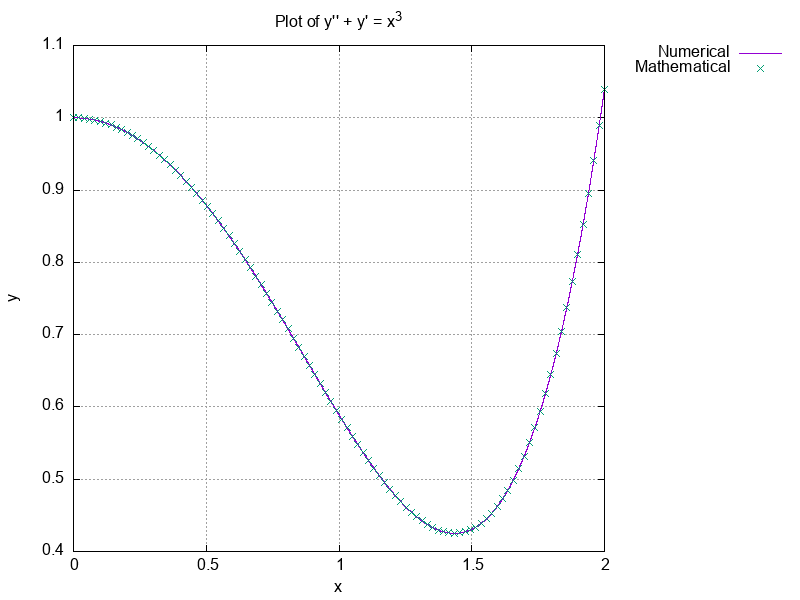
\includegraphics[width=1\textwidth]{./plot.png}
\end{center}
Since the solutions from power series and Laplace are the same, we define one function to represent them and plot as points. We can see the line tracks perfectly along the points, so the two results are equivalent. 

\section*{Conclusion}
Solving $y'' + y = x^3$ with power series, Laplace transforms, and the numerical method with C programs all result in the same answer. The numerical method is short and sweet, and can easily solve differential equations, assuming you have a computer and can write C.


\end{document}
